%%%%%%%%%%%%%%%%%%%%%%%%%%%%%%%%%%%%%%
%
%          TITLE AND AUTHORS
%
%%%%%%%%%%%%%%%%%%%%%%%%%%%%%%%%%%%%%%%


\chapter{The Impact of Accretion Disc Winds on the Optical Spectra of Cataclysmic Variables}

{\em This chapter is based on the publication:

Matthews J. H., Knigge C., Long K. S., Sim S. A., Higginbottom N., 
`The impact of accretion disc winds on the optical spectra of 
cataclysmic variables',
2015, MNRAS, 450, 3331.}
%%%%%%%%%%%%%%%%%%%%%%%%%%%%%%%%%%%%%%
%
%          INTRODUCTION
%
%%%%%%%%%%%%%%%%%%%%%%%%%%%%%%%%%%%%%%%

\section{Introduction} 
\label{sec:intro}

% \begin{figure*}
% \centering
% 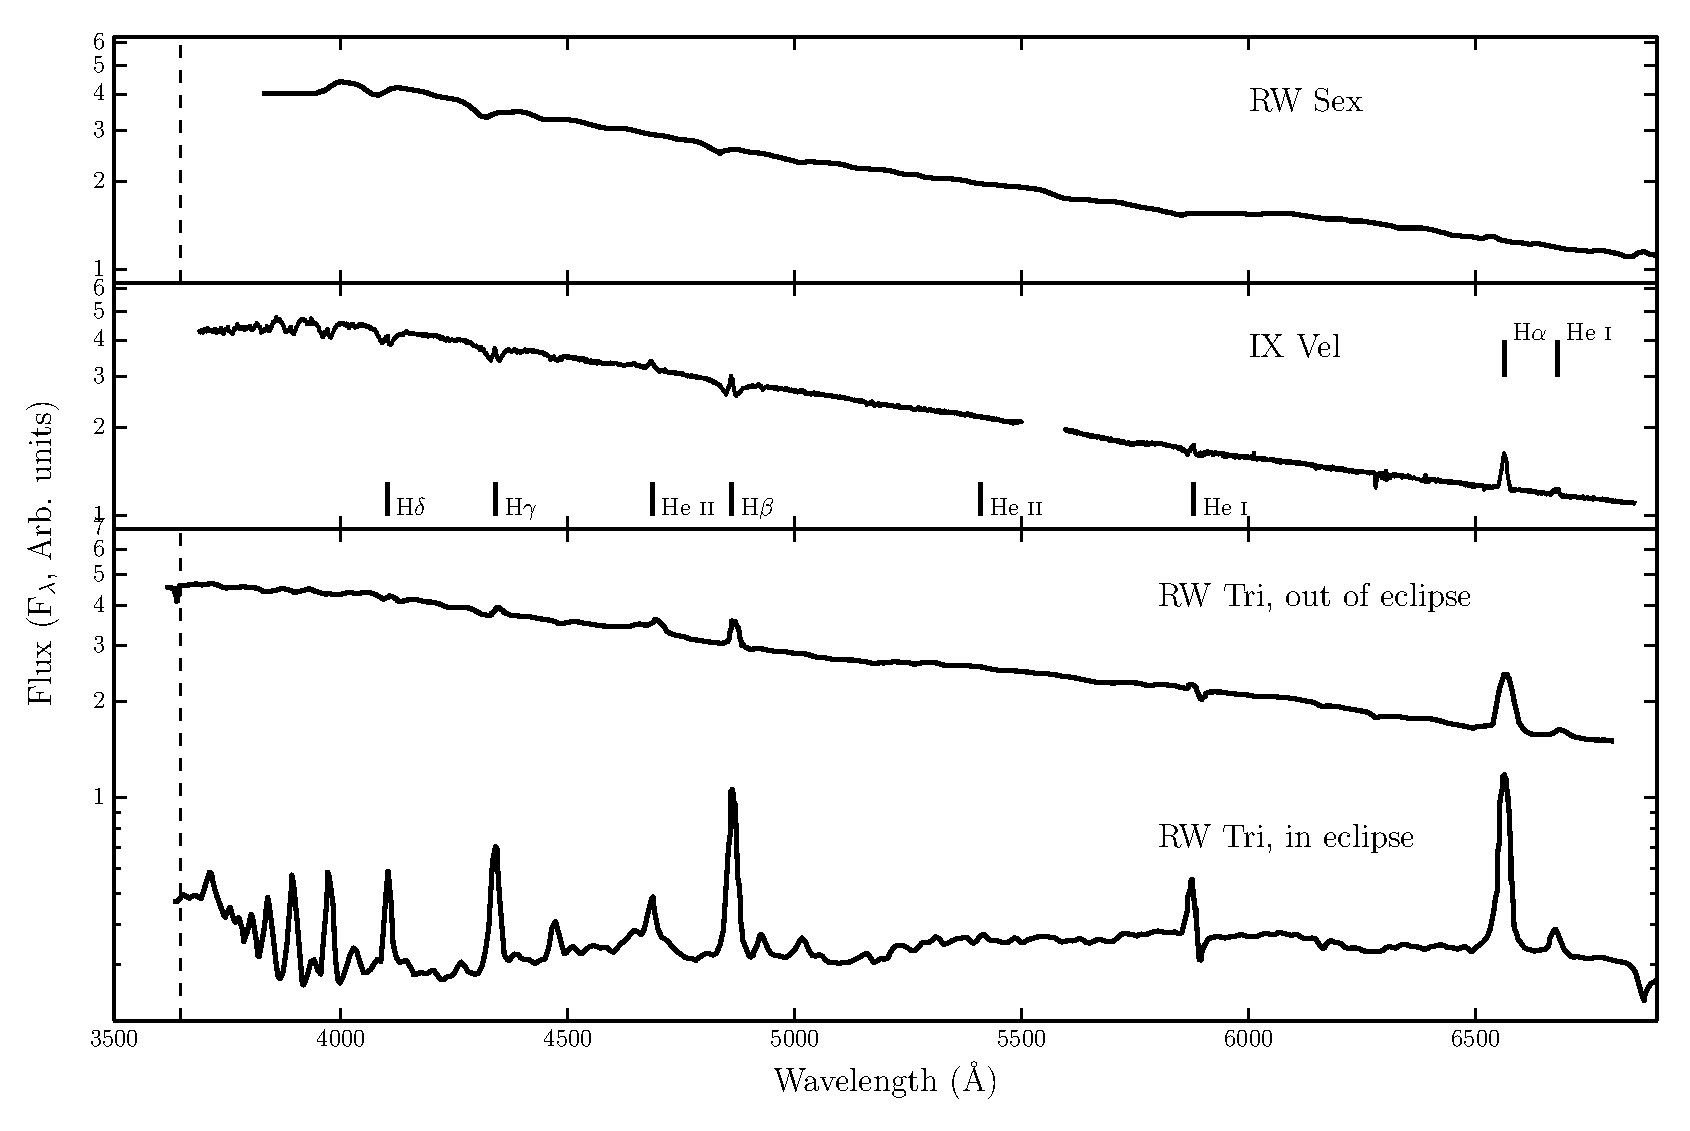
\includegraphics[width=1.0\textwidth]{figures/05-cvpaper/fig1.eps}
% \caption
% [Optical spectra of three nova-like variables]
% {
% Optical spectra of three nova-like variables: 
% RW Sex (top; Beuermann et al. 1992),
% IX Vel (top middle; A. F. Pala \& B. T. Gaensicke, private communication) 
% and RW Tri in and out of eclipse (bottom two panels; Groot et al. 2004).
% The data for RW Sex and RW Tri were digitized from the respective publications,
% and the IX Vel spectrum was obtained using the XSHOOTER spectrograph 
% on the Very Large Telescope on 2014 October 10.
% These systems have approximate inclinations of $30^\circ$, $60^\circ$ and $80^\circ$ 
% (see section 5.4) respectively. 
% The trend of increasing Balmer line emission with inclination can be seen.
% In RW Tri strong single-peaked emission in the Balmer lines is seen even
% in eclipse, indicating that the lines may be formed in a spatially
% extensive disc wind, and there is even a suggestion 
% of a (potentially wind-formed) recombination continuum in the eclipsed
% spectrum. We have attempted to show each spectrum over a similar dynamic range.
% }
% \label{novalikes}
% \end{figure*}


% It has been known for a long time that winds emanating from the
% accretion disc are important in shaping the ultraviolet (UV) spectra
% of high-state CVs \citep{heap1978, greensteinoke1982}. The most spectacular evidence for such
% outflows are the P-Cygni-like profiles seen in UV resonance lines such as
% \civfull\ (see e.g. Cordova \& Mason
% 1982\nocite{cordova1982}). Considerable effort has been spent over the
% years on understanding and modelling these UV features (e.g. Drew \&
% Verbunt 1985\nocite{drewverbunt1985}; Mauche \& Raymond
% 1987\nocite{maucheraymond1987}; Drew 1987; Shlosman \& Vitello 1993; [hereafter
% SV93]\nocite{SV93}; Knigge, Woods \& Drew 1995\nocite{KWD95}; 
% Knigge \& Drew 1997\nocite{kd1997}; 
% Knigge et al. 1997\nocite{knigge1997}; Long \& Knigge 2002 [hereafter LK02]\nocite{LK02}, 
% Noebauer et al. 2010\nocite{noebauer};
% Puebla et al. 2011\nocite{puebla2011}). The basic picture emerging from these efforts is
% of a slowly accelerating, moderately collimated bipolar
% outflow that carries away $\simeq 1\% - 10\%$ of the accreting
% material. State-of-the-art simulations of line formation in this type
% of disc wind can produce UV line profiles that are remarkably similar
% to observations.

% Much less is known about the effect of these outflows on the optical
% spectra of high-state CVs. These spectra are typically characterized
% by H and He emission lines superposed on a blue continuum. In many
% cases, and particularly in the SW~Sex subclass of NLs
% \citep{HSK86,DR95}, these lines are single-peaked. This is contrary to
% theoretical expectations for lines formed in accretion discs, which
% are predicted to be double-peaked \citep{smak1981, hornemarsh1986}. 
% {\em Low-state} CVs (dwarf novae in quiescence) do, in fact,
% exhibit such double-peaked lines \citep{marshhorne1990}. 

% Murray \& Chiang (1996, 1997; hereafter referred to collectively as MC96)\nocite{MC96, MC97} 
% have shown that the presence of disc winds may
% offer a natural explanation for the single-peaked optical emission lines in
% high-state CVs, since they can strongly affect the radiative transfer
% of line photons. Strong support for a significant wind contribution to the
% optical emission lines comes from observations of eclipsing
% systems. There, the single-peaked lines are often only weakly
% eclipsed, and a significant fraction of the line flux remains visible
% even near mid-eclipse \citep[e.g.][]{baptista2000,groot2004}. 
% This points to line formation in a spatially
% extended region, such as a disc wind (see Fig.~\ref{novalikes}).
% %%(Honeycutt, Schlegel, \& Kaitchuck 1986; Dhillon \& Rutten 1995). 
% Further evidence for a wind contribution to the optical lines comes
% from isolated observations of P-Cygni-like line profiles even in optical
% lines, such as \ha\ and He \textsc{i} $\lambda5876$ \citep{patterson1996, RN98, kafka2004}.

% Could disc winds also have an impact on the UV/optical {\em continuum}
% of high-state CVs? This continuum is usually thought to be dominated
% by the accretion disc and modelled by splitting the disc into
% a set of concentric, optically thick, non-interacting annuli following
% the standard $T_{eff}(R) \propto R^{-3/4}$ radial temperature
% distribution \citep{shakurasunyaev1973}. In such
% models, each annulus is taken to emit either as a blackbody or,
% perhaps more realistically, as a stellar/disc atmosphere model
% \citep{Schwarzenberg-Czerny1977,wade1984,wade1988}.
% In the latter case, the local surface gravity, $\log{g}(R)$, is
% assumed to be set solely by the accreting WD, since self-gravity is
% negligible in CV discs.

% Attempts to fit the observed spectral energy distributions (SEDs) of
% high-state CVs with such models have met with mixed success. In
% particular, the SEDs predicted by most stellar/disc atmosphere models 
% are too blue in the UV \citep{wade1988,long1991,long1994,knigge1998} and exhibit
% stronger-than-observed Balmer jumps in absorption 
% \citep{wade1984,haug1987,ladous1989b,knigge1998}. One possible
% explanation for these problems is that these models fail to capture
% all of the relevant physics. Indeed, it has been argued that a
% self-consistent treatment can 
% produce better agreement with observational data (e.g. Shaviv et
% al. 1991;  but see also Idan et al. 2010).
% \nocite{idanshaviv2010} \nocite{shaviv1991}
% However, an alternative explanation, suggested by Knigge et al.
% (1998b; see also Hassall et al. 1985)\nocite{KLWB98,hassall}, 
% is that recombination continuum emission from the base of the 
% disc wind might fill in the disc's
% Balmer absorption edge and flatten the UV spectrum. 

\nocite{groot2004}
\nocite{beuermann1990}
\nocite{beuermann1992}
\nocite{higginbottom2013}

Here, I present Monte Carlo radiative transfer simulations designed
to assess the likely impact of accretion disc winds on the
optical spectra of high-state CVs. The goal is to
test whether the disc winds that produce the UV
resonance lines also naturally produce significant amounts of  
optical emission. More specifically, I aim to investigate whether a 
disc wind model can reproduce the optical lines observed in CV spectra,
such as \ha, \hb, \heiiopt\ and the He~\textsc{i} lines, as well as
the \heiiuv\ emission line. I also aim to explore whether the recombination
continuum from the wind can sucessfully `fill-in' the Balmer photoabsorption
edge intrinsic to stellar or disc atmosphere spectra, and establish
if a disc wind model can produce single-peaked lines as proposed
by \cite[][hereafter referred to collectively as MC96]{MC96,MC97}.
The relevant background to this study is outlined in section~\ref{sec:cv_winds}.

In order to carry out these simulations and effectively model the optical
spectra of CVs, I use the `macro-atom' approach described in chapter 3. 
With this method, \py\ is able to deal correctly with processes involving
excited levels, such as the recombination emission observed in CV spectra.
The prescription used to describe the wind is the biconical SV93 model described in 
section~\ref{sec:sv93_model}; a schematic for this specific application
is shown in Fig.~\ref{cartoon}. The remainder of this chapter is organized as follows. I begin
by describing the photon sources and input SED used in this modelling.
In section~\ref{modela}, I present spectra simulated from the benchmark 
model employed by LK02. In section~\ref{sec:modelb}, I present a revised model
optimized for the optical waveband, before summarising the
findings in section~\ref{sec:cv_conclusions}.


\subsection{Sources and Sinks of Radiation}
\label{radsources}

\begin{figure} 
\centering
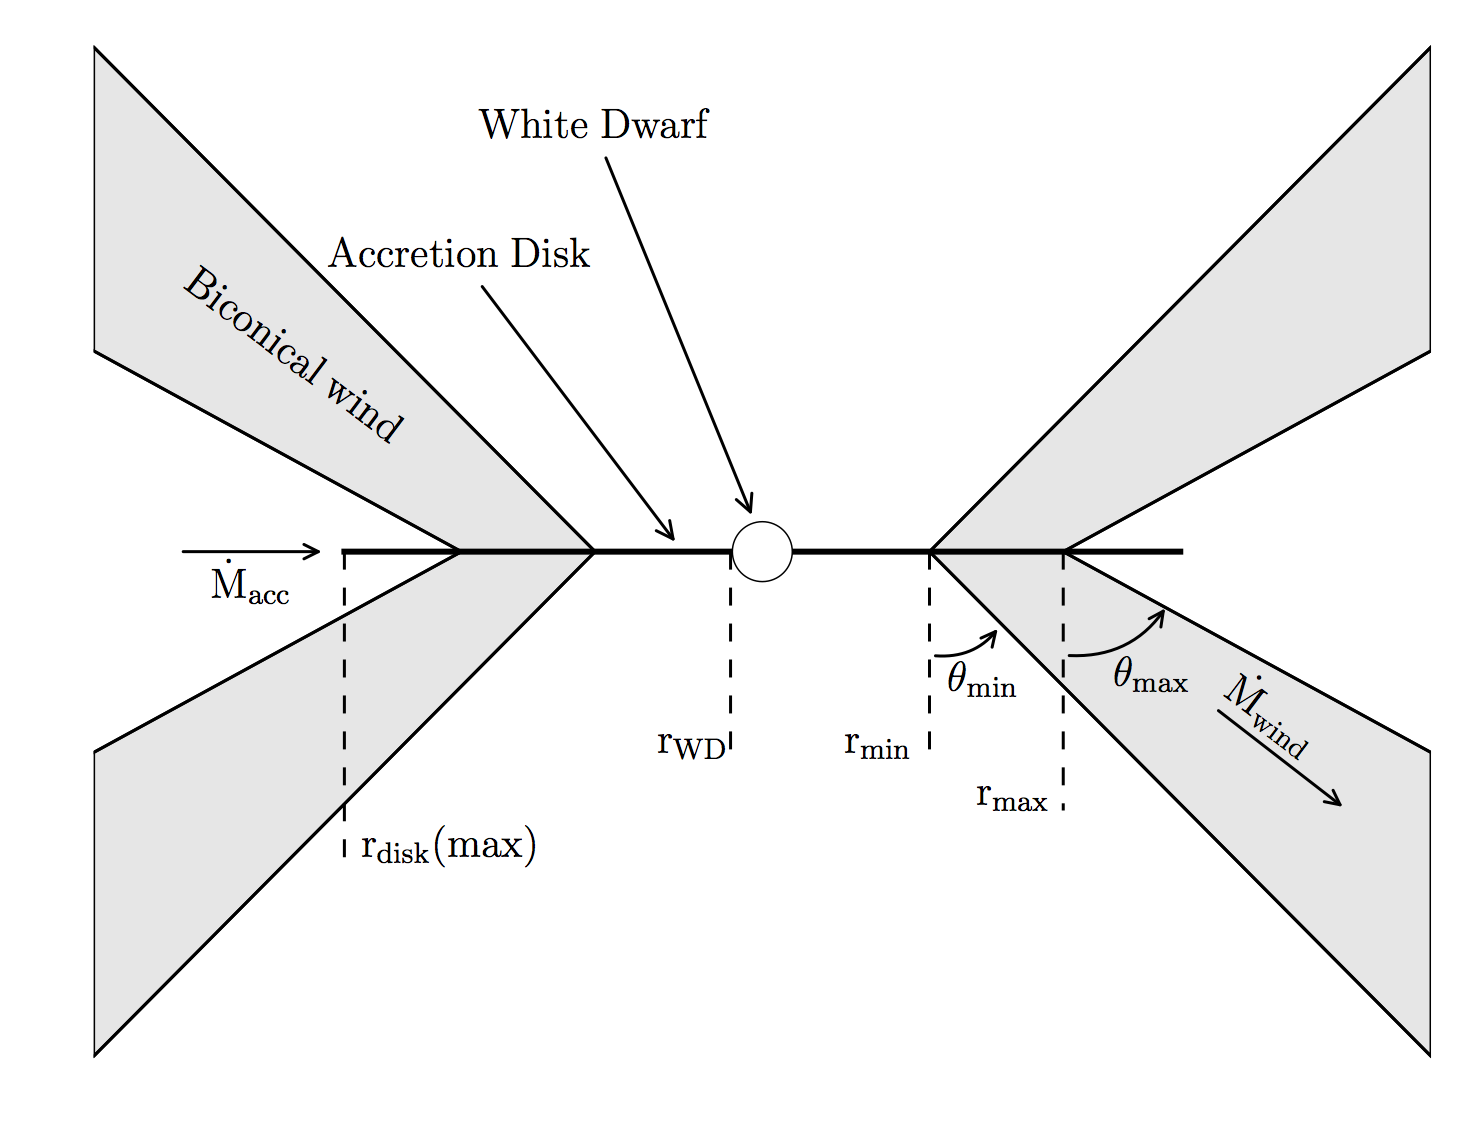
\includegraphics[width=1.0\textwidth]{figures/05-cvpaper/fig2_cartoon.png}
\caption{Cartoon illustrating the geometry and kinematics of the benchmark CV wind model.}
\label{cartoon}
\end{figure} 

The net photon sources in this CV model are the accretion disc, the
WD and, in principle, a boundary layer with user-defined temperature
and luminosity. All of these radiating bodies are taken to be
optically thick, and photons striking them are assumed to be destroyed
instantaneously. The secondary star is not included as a radiation
source, but is included as an occulting body. This allows us to model
eclipses. Finally, emission from the wind itself is also accounted for, but
note that this assumes the outflow is in radiative equilibrium. Thus all
of the heating of the wind, as well as its emission, is ultimately
powered by the radiation field of the net photon sources in the
simulation. In the following sections, I will describe the treatment
of these system components in slightly more detail, which are also
shown in Fig.~\ref{cartoon}.

\subsubsection{Accretion disc}

\py\ has some flexibility when treating the accretion 
disc as a source of photons. The disc is broken down into annuli 
such that each annulus contributes an equal amount to the bolometric
luminosity. The disc is taken to be geometrically thin, but optically
thick, and I thus adopt the temperature profile of a standard
\cite{shakurasunyaev1973} $\alpha$-disc. An annulus can then
be treated either as a blackbody with the corresponding effective
temperature or as a stellar atmosphere model with the appropriate
surface gravity and effective temperature. Here, blackbodies are used
during the ionization cycles and to compute the Monte Carlo
estimators. The input SED for the ionization cycles is shown in 
Fig.~\ref{cv_model_sed}
However, during the spectral synthesis stage of the 
simulation stellar atmosphere models are used. This produces more
realistic model spectra and allows us to test if recombination
emission from the wind base can fill in the Balmer jump, which is
always in absorption in these models. The synthetic stellar atmosphere
spectra are calculated with
\textsc{Synspec}\footnote{http://nova.astro.umd.edu/Synspec43/synspec.html}
from either Kurucz \citep{kurucz1991} atmospheres (for $T_{\mathrm{eff}} \leq
50,000$~K) or from \textsc{TLUSTY} \citep{tlusty} models (for $T_{\mathrm{eff}} > 50,000$~K). 

\begin{figure} 
\centering
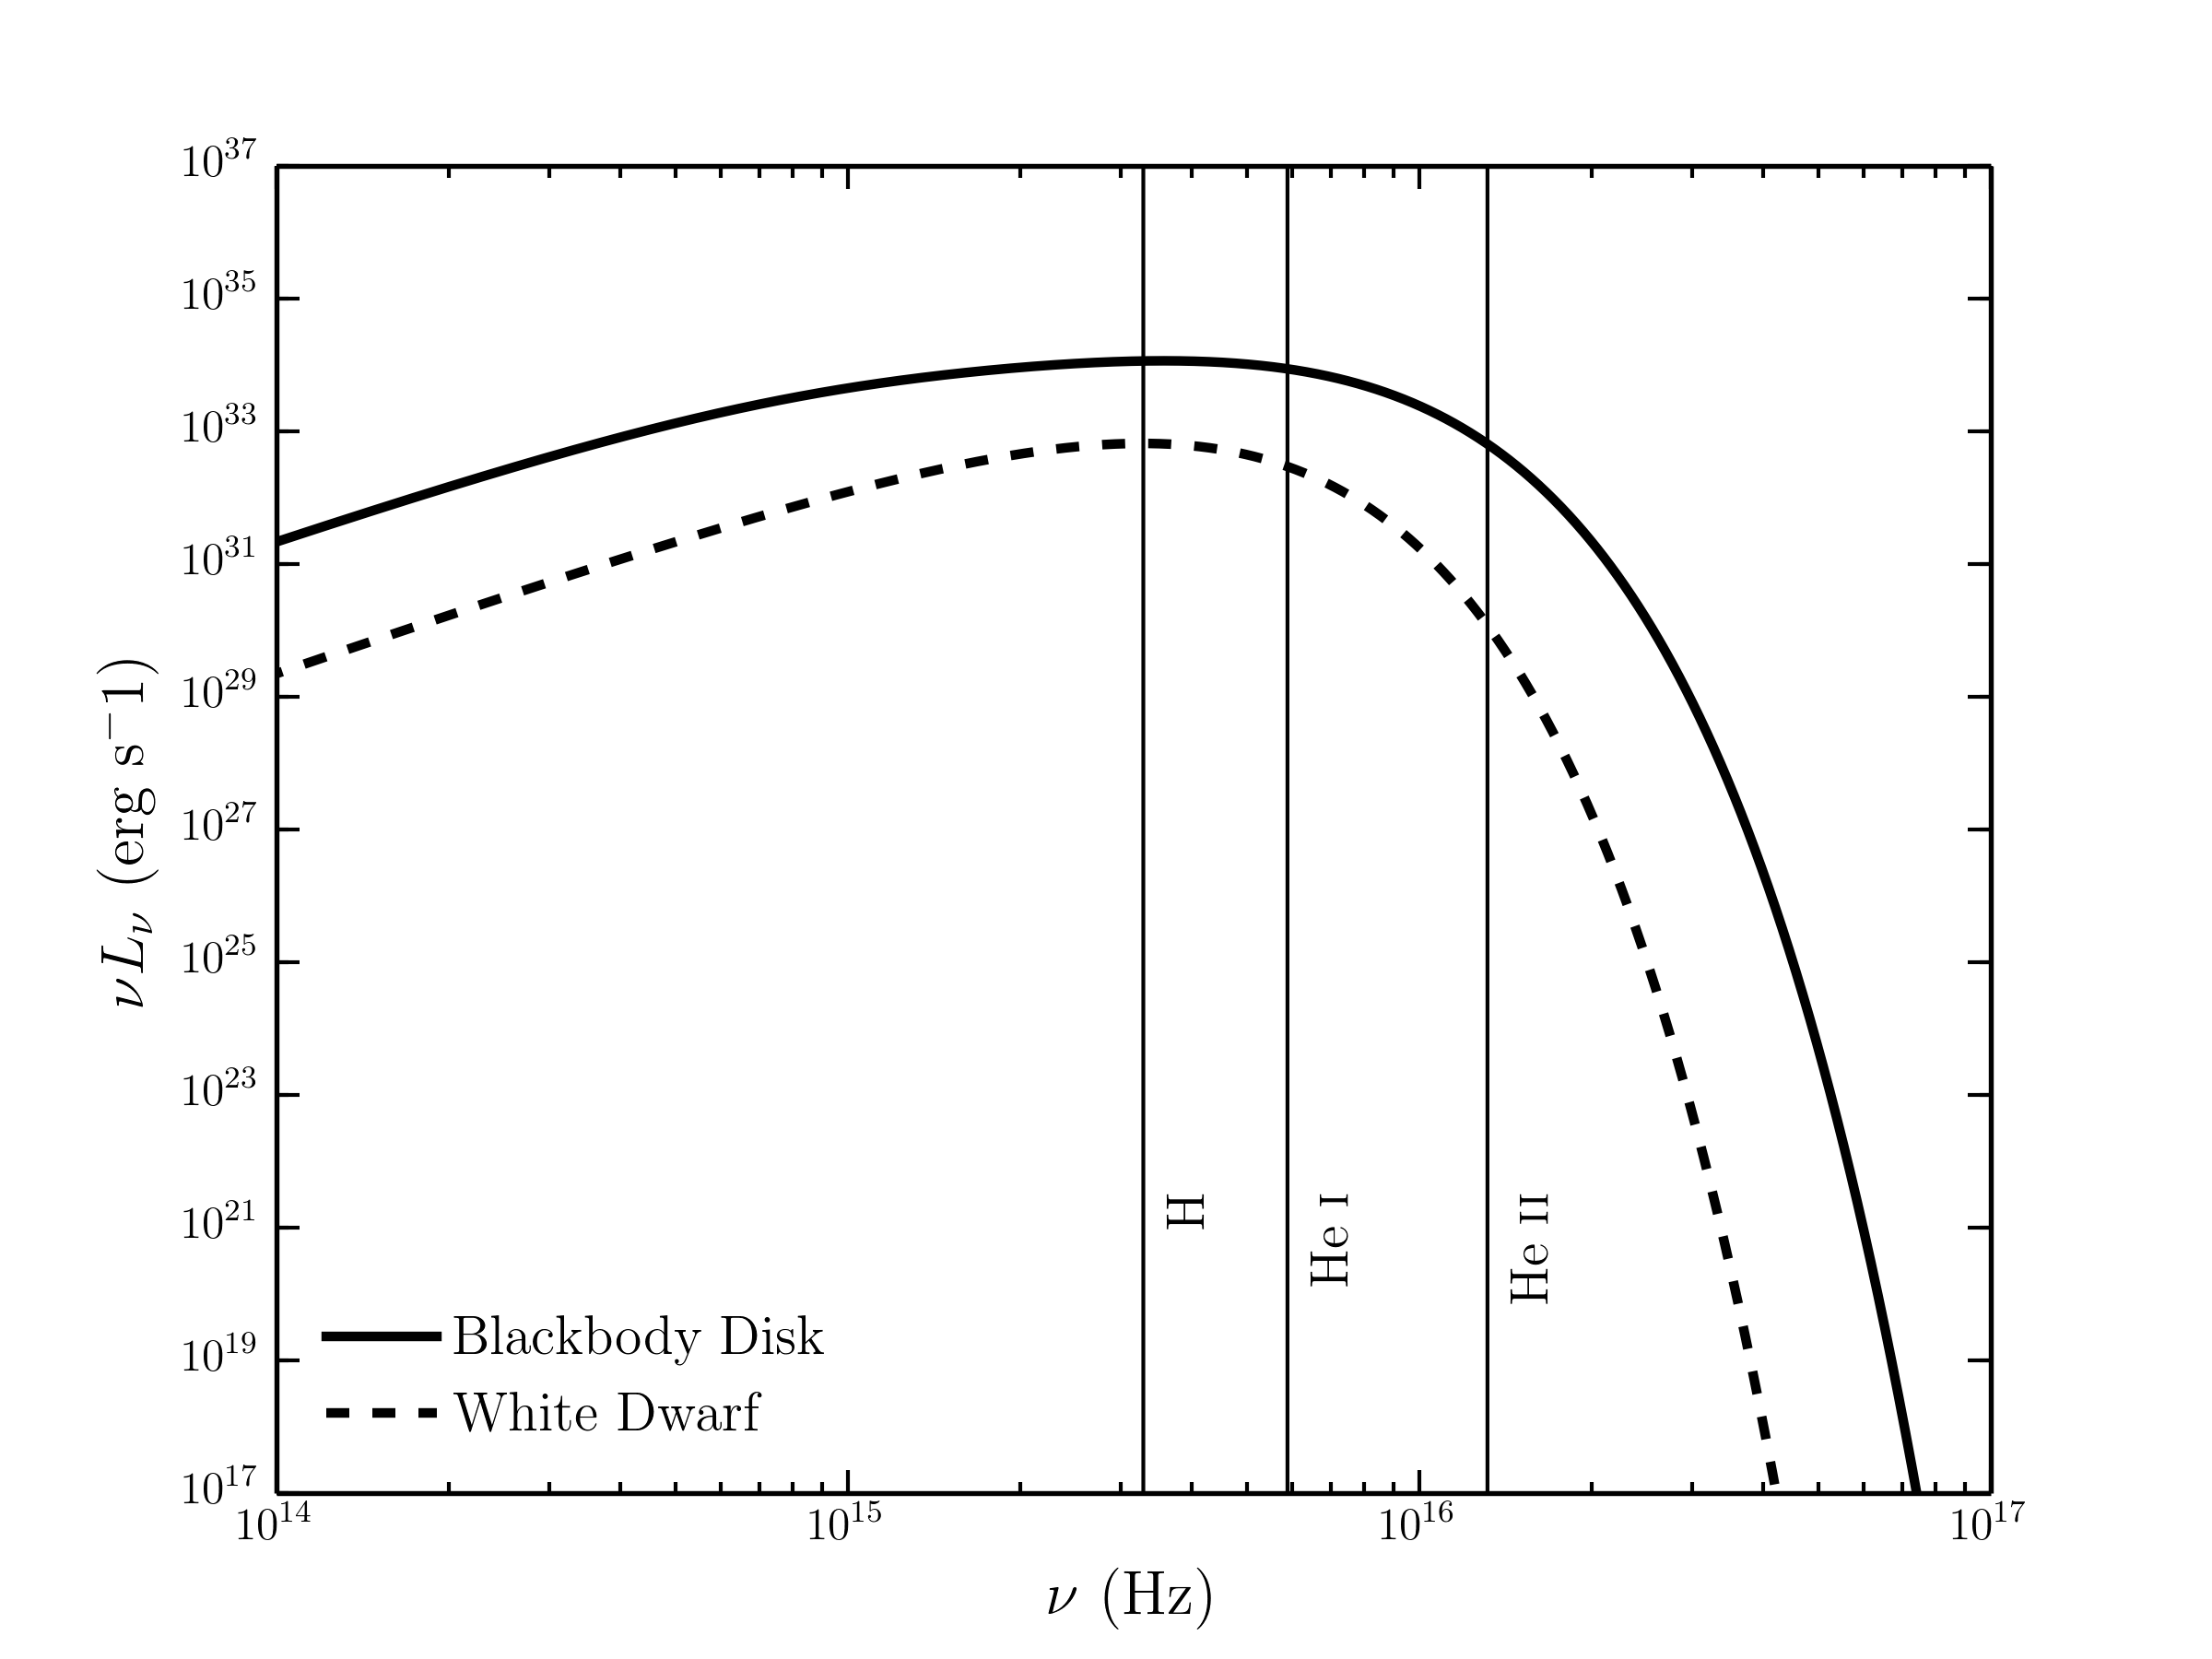
\includegraphics[width=0.8\textwidth]{figures/05-cvpaper/sed.png}
\caption{The spectral energy distribution of the 
accretion disc and white dwarf used in the ionization cycles for
the CV modelling. The important ionization edges for
hydrogen and helium are marked.}
\label{cv_model_sed}
\end{figure} 

\subsubsection{White Dwarf}

The WD at the center of the disc is always present as a spherical occulting
body with radius $R_{WD}$ in \py\ CV models, but it can also be included
as a source of radiation. In the models presented here,the
WD is treated as a blackbody radiator with temperature $T_{WD}$ and luminosity
$L_{WD} = 4\pi R_{WD}^2 \sigma T_{WD}^4$. 

\subsubsection{Boundary Layer}

It is possible to include radiation from a boundary layer (BL) between
the disc and the WD. In \py, the BL is described as
a blackbody with a user-specified effective temperature and
luminosity. The models presented here initially follow LK02 in setting
the BL luminosity to zero, partly as the temperature, luminosity, and even
existence of a BL in CVs with strong winds is not certain \citep{hoaredrew1993}.
However, I have confirmed that the addition 
of an isotropic BL with $L_{BL} = 0.5 L_{\mathrm{acc}}$ and temperatures in 
the range $80~{\rm kK} \leq T_{BL} \leq 200~{\rm kK}$ would not change 
any of the main conclusions here. 
The influence of the BL on the heating and cooling balance
in the wind, as well as the emergent spectrum, is briefly discussed in
section~\ref{sec:coll_bl}.


\subsubsection{Secondary Star}

The donor star is included in the system as a pure radiation sink, 
i.e. it does not emit photons, but absorbs any photons that strike its
surface. The secondary is assumed to be Roche-lobe filling, so its
shape and relative size are defined by setting the mass ratio of the system, 
$q_M = M_2/M_{WD}$. The inclusion of the donor star as an occulting body
allows us to model eclipses of the disc and the wind. For this
purpose, I assume a circular orbit with a semi-major axis $a$ and 
specify orbital phase such that $\Phi_{\mathrm{orb}} = 0$ is the
inferior conjunction of the secondary (i.e. mid-eclipse for $i \simeq
90^\circ$).




%%%%%%%%%%%%%%%%%%%%%%%%%%%%%%%%%%%%%%
%
%          BENCHMARK MODEL
%
%%%%%%%%%%%%%%%%%%%%%%%%%%%%%%%%%%%%%%%


\begin{table}
\centering
\begin{tabular}{p{2cm}p{2cm}p{2cm}}
%\multicolumn{2}{l}{Model Parameters}  \\
%%Model Parameters \\
\hline Parameter 	&	 Model A  & Model B \\ 
\hline \hline 
$M_{WD}$ 	 &	 $0.8~M_{\odot}$  &     \\ 
$R_{WD}$ 	 &	 $7\times10^{8}$~cm  & \\ 
$T_{WD}$ 	 &	 $40,000$~K        &  \\
$M_{2}$ 	& -&	 $0.6~M_{\odot}$   \\ 
$q_M$ 	&- &	 $0.75$   \\ 
$P_{\mathrm{orb}}$ 	&- &	 $5.57$~hr   \\ 
$a$ 	& -&	 $194.4~R_{WD}$   \\ 
$R_2$   &   -  &	 $69.0~R_{WD}$  \\ 
$\dot{M}_{\mathrm{acc}}$ 	 &	 $10^{-8}~M_{\odot}yr^{-1}$  &\\ 
$\dot{M}_W$  &	$10^{-9}~M_{\odot}yr^{-1}$å  & \\ 
$r_{\mathrm{min}}$ 	&	 $4~R_{WD}$ &  \\ 
$r_{\mathrm{min}}$ 	&	 $12~R_{WD}$  &  \\ 
$r_{\mathrm{disc}}$(max) 	&	 $34.3~R_{WD}$  &  \\ 
$\theta_{\mathrm{min}}$	&	 $20.0^{\circ}$  &  \\ 
$\theta_{\mathrm{max}}$ 	&	 $65.0^{\circ}$  &  \\ 
$\gamma$ 	&	 $1$  &  \\ 
$v_{\infty}$ 	&	 $3~v_{\mathrm{esc}}$  &  \\ 
$R_v$ 	        &	 $100~R_{WD}$  &  $142.9~R_{WD}$  \\ 
$\alpha$ 	&	 $1.5$   &   $4$\\
\hline 
\end{tabular} 
\centering
\caption
[Model parameters for the CV wind models]
{
Parameters used for the geometry and kinematics of the benchmark 
CV model (model A), which is optimized for the UV band, and a model
which is optimized for the optical band and described in section~\ref{sec:modelb} (model B).
For model B, only parameters which are altered are given - otherwise the
model A parameter is used. $P_{\mathrm{orb}}$ is the orbital period 
(the value for RW Tri from Walker 1963 is adopted, see section~\ref{sec:rwtri}) and 
$R_2$ is the radius of a sphere with the volume of the secondary's Roche lobe. 
Other quantities are defined in the text or Fig.~\ref{cartoon}.
Secondary star parameters are only quoted for 
model B as I do not show eclipses with the 
benchmark model (see section~\ref{sec:rwtri}).
}
\label{wind_param}
\label{modelb_table}
\end{table}

\nocite{walker1963}

\section{A Benchmark Disc Wind Model}
\label{modela}

The main goal is to test whether the type of disc wind model that has
been successful in explaining the UV spectra of CVs could also have a
significant impact on the optical continuum and emission line spectra
of these systems. In order to set a benchmark, I therefore begin by
investigating one of the fiducial CV wind models that was used by SV93
and LK02 to simulate the UV spectrum of a typical high-state
system. The specific parameters for this model (model A) are listed in
Table~1. A key point is that the wind mass-loss rate in this model is
set to 10$\%$ of the accretion rate through the disc. I follow SV93
in setting the inner edge of the wind ($r_{\mathrm{min}}$) to $4~R_{WD}$. 
The sensitivity to some of these parameters is briefly discussed in
section~\ref{sec:cv_params}. 

\subsection{Physical Structure and Ionization State}
\label{modela_ionization}

\begin{figure*}
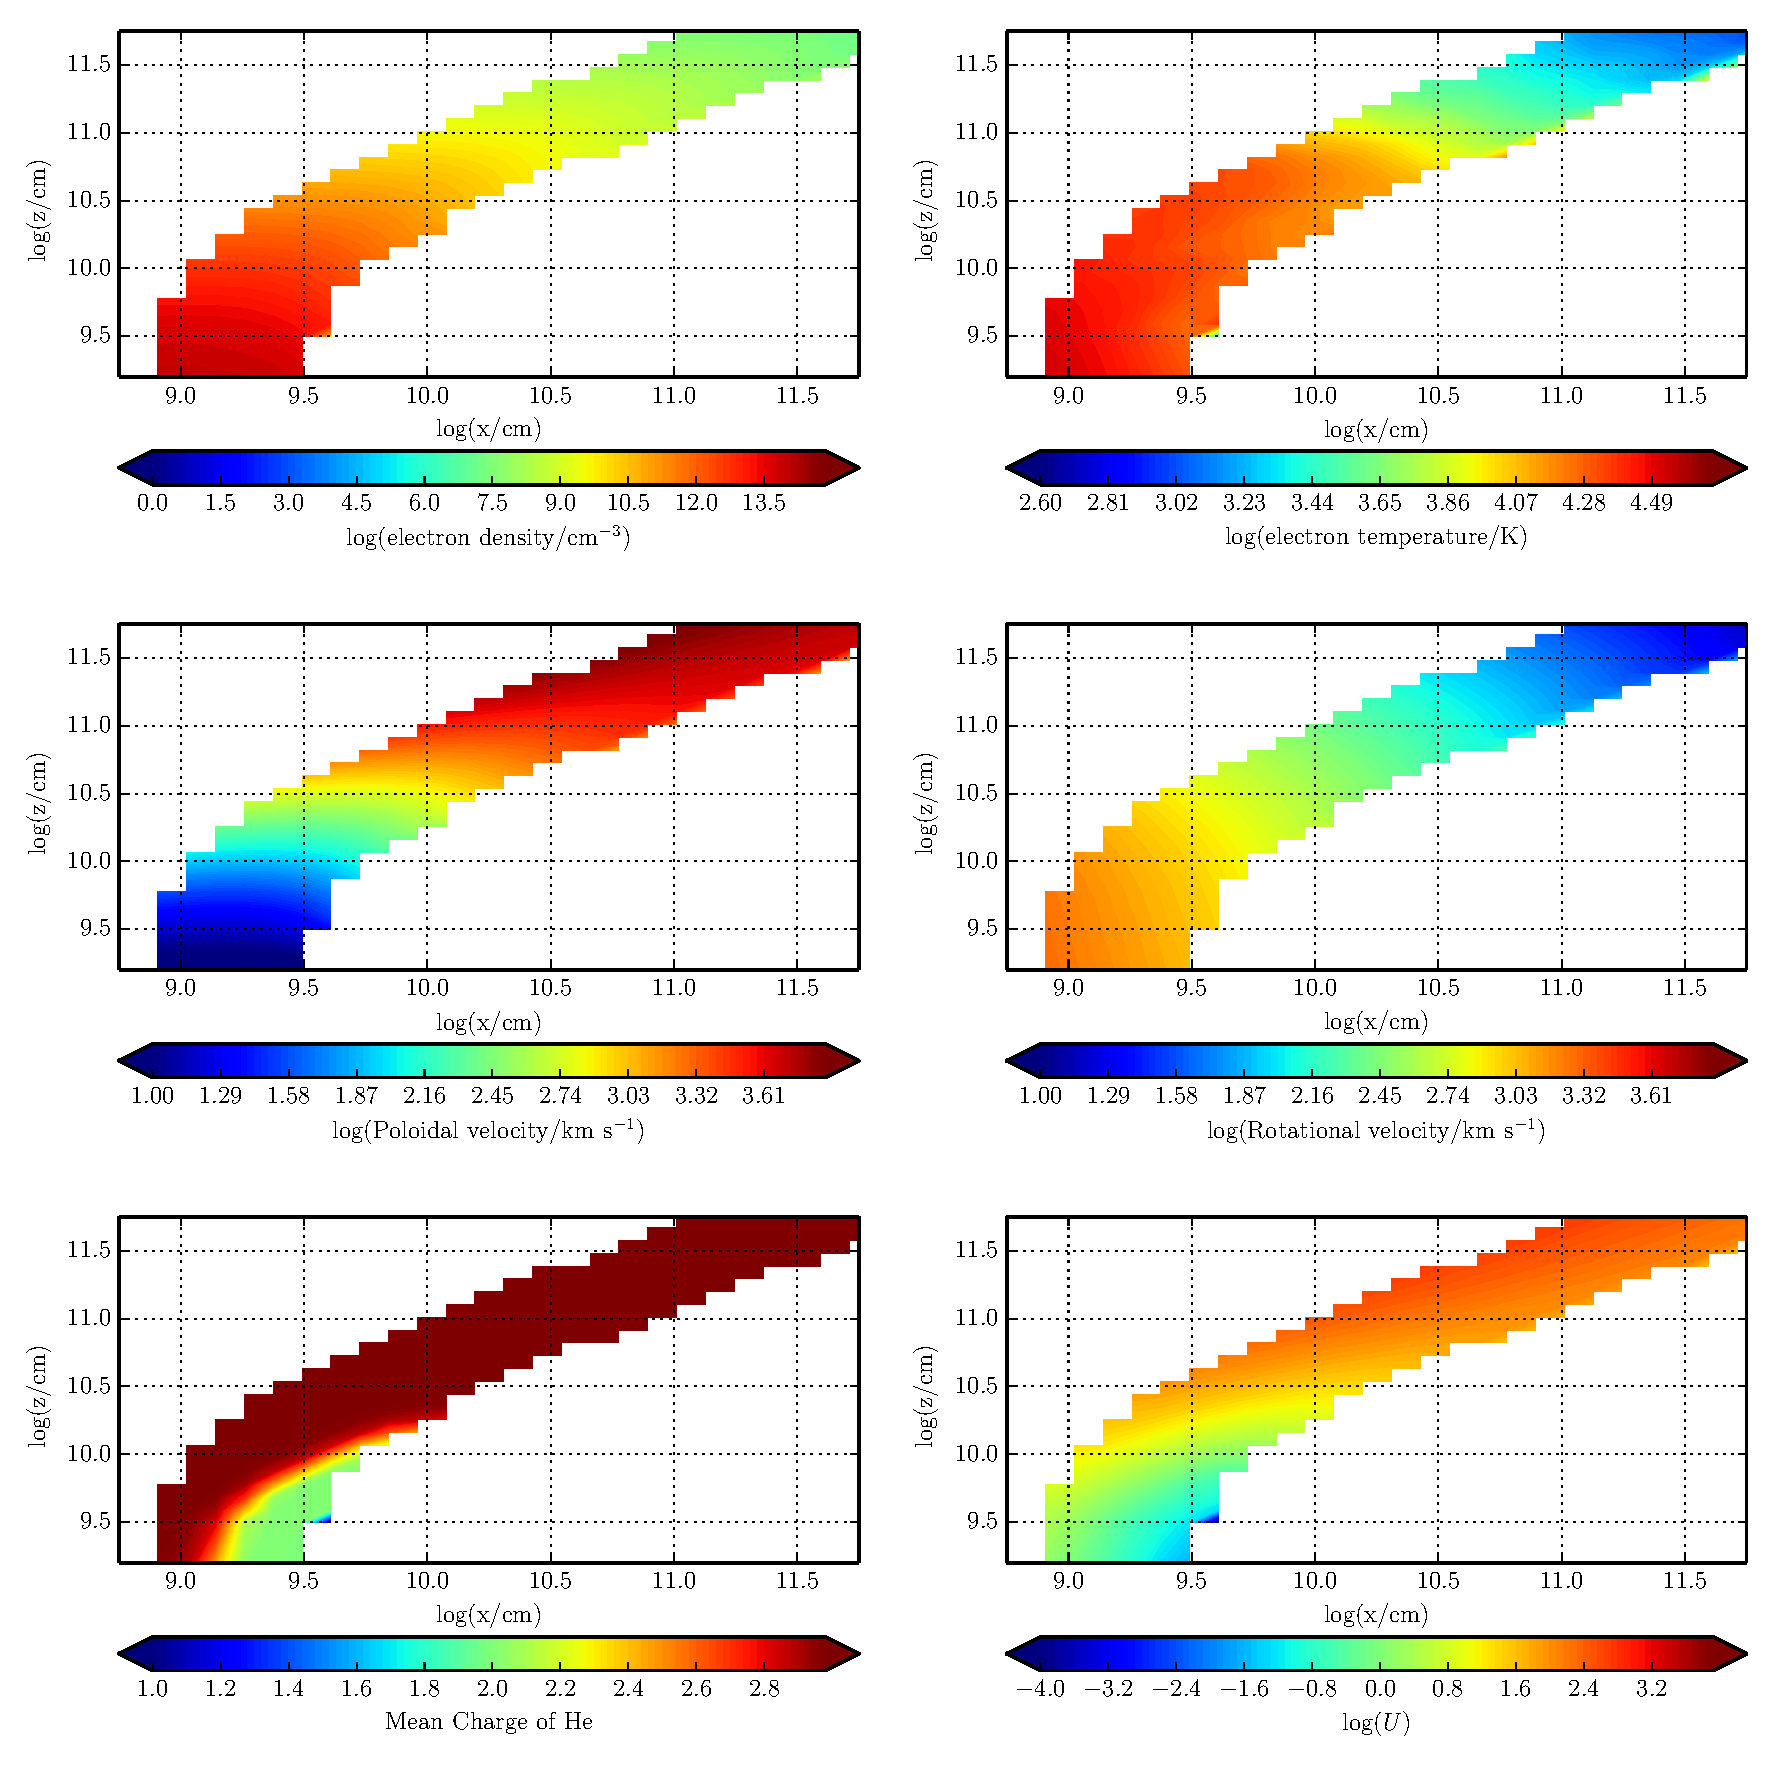
\includegraphics[width=1.0\textwidth]{figures/05-cvpaper/fig5.eps}
\caption
[The physical properties of the wind in the benchmark CV model.]
{
The physical properties of the wind -- note the logarithmic scale. 
Near the disc plane the wind is dense, with low poloidal velocities.
As the wind accelerates it becomes less dense
and more highly ionized. The dominant He ion
is almost always He III, apart from in a small
portion of the wind at the base, which is partially shielded
from the inner disc.
}
\label{wind}
\end{figure*}

Fig.~\ref{wind} shows the physical and ionization structure 
of the benchmark disc wind model. The ionization parameter shown in the bottom
right panel is given by equation~\ref{eq:ip}
 The ionization parameter is a useful measure of the ionization state of a plasma, 
as it evaluates the ratio of the number density of ionizing photons to the local 
H density.

There is an obvious drop-off in density
and temperature with distance away from the disc, so any line
formation process that scales as $\rho^2$ -- i.e. recombination and
collisionally excited emission -- should be expected to operate
primarily in the dense base of the outflow. Moreover, a comparison of
the rotational and poloidal velocity fields shows that rotation
dominates in the near-disc regime, while outflow dominates further out
in the wind. 

The ionization equation used in the `simple atom' approach used by
LK02 (see section~\ref{sec:simple_ionization}) should be a reasonable approximation to
the photoionization equilibrium in the benchmark wind model. Even
though the macro-atom treatment of H and He does affect the 
computation of the overall ionization equilibrium, the
resulting ionization state of the wind should be similar to that
found by LK02. The bottom panels in Fig.~\ref{wind} confirm that this
is the case. In particular, He is fully ionized
throughout most of the outflow, except for a small region near the
base of the wind, which is shielded from the photons produced by the
hot inner disc. In line with the results of LK02,
C\textsc{iv} is the dominant C ion throughout the wind,
resulting in a substantial absorbing column across a large range of
velocities. As we shall see, this produces the broad, deep and
blue-shifted C\textsc{iv}~$\lambda1550$ absorption line that
is usually the most prominent wind-formed feature in the UV spectra of
low-inclination nova-like CVs.

\begin{figure*}
\centering
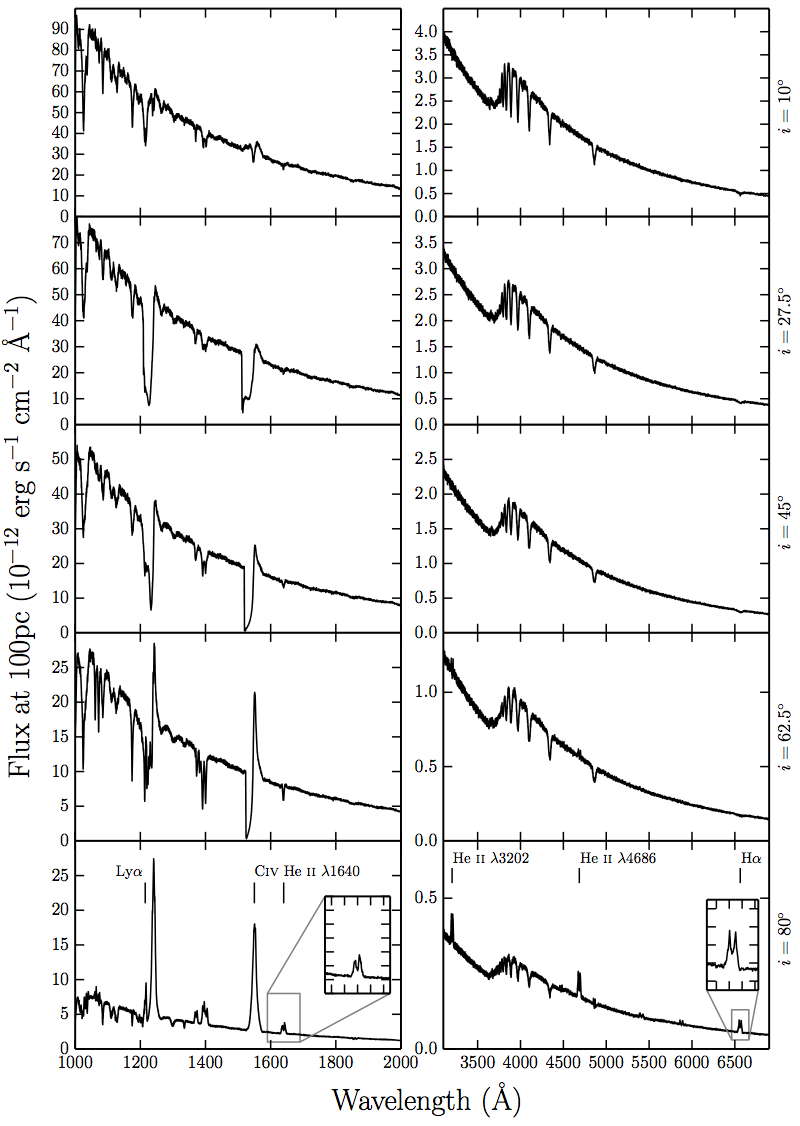
\includegraphics[width=1.0\textwidth]{figures/05-cvpaper/modela_uv_opt.png}
\caption
[UV and optical synthetic spectra from the benchmark CV model]{
UV (left) and optical (right) synthetic spectra for model A, the benchmark model,
computed at sightlines of 10, 27.5, 45, 62.5 and 80 degrees.	
The inset plots show zoomed-in line profiles for 
\heiiuv\ and \ha. Double-peaked line emission can be seen in 
\heiiuv, \heiiopt, \ha\ and some He I lines, but the 
line emission is not always sufficient to overcome the absorption
cores from the stellar atmosphere models. The model
also produces a prominent \heiioptnew\ line at high inclinations.
}
\label{spec}
\end{figure*}



\subsection{Synthetic Spectra}
\label{modela_spectrum}
\label{sec:modela_spectra}

I begin by verifying that the benchmark model still produces UV
spectra that resemble those observed in CVs. This should be
the case, since the ionization state of the wind has not changed
significantly from that computed by LK02 (see section~\ref{modela_ionization}). 
The left column of panels in Fig.~\ref{spec} shows that this expectation
is met: all of the strong metal resonance
lines -- notably N~\textsc{v}~$\lambda1240$,
Si~\textsc{iv}~$\lambda1400$ and C~\textsc{iv}~$\lambda1550$ -- 
are present and exhibit clear P-Cygni profiles
at intermediate inclinations. In addition, however, I now also find
that the wind produces significant Ly$\alpha$ and
He~\textsc{ii}~$\lambda1640$ emission lines. 

Fig.~\ref{spec} (right-hand panel) and Fig.~\ref{spec_continuum}
show the corresponding optical spectra produced for
the benchmark model, and these do exhibit some emission lines
associated with H and He. There is 
a general trend from absorption lines to emission lines 
with increasing inclination, as we might expect from this wind
geometry. This trend is consistent with observations, as can be seen
in Fig.~1. However, it is clear that this particular model
does not produce all of the lines seen in observations of high-state CVs.
The higher-order Balmer series lines are too weak
to overcome the intrinsic absorption from the disc atmosphere, and the wind 
fails to produce any observable emission at low and intermediate inclinations.
This contrasts with the fact that emission lines are seen 
in the optical spectra of (for example) V3885 Sgr \citep{hartley2005}
and IX Vel \citep[][see also Fig.~1]{beuermann1990}.

The emissivity of these recombination 
features scales as $\rho^2$, meaning that they form almost entirely in the 
dense base of the wind, just above the accretion disc. Here, the
velocity field of the wind is still dominated by rotation, rather than
outflow, which accounts for the double-peaked shape of the lines. In
principle, lines formed in this region can still be single peaked,
since the existence of a poloidal velocity {\em gradient} changes the
local escape probabilities (MC96). However, as
discussed further in section~\ref{sec:cv_line_shapes}, the 
radial velocity shear in the
models is not high enough for this radiative transfer effect
to dominate the line shapes.

The Balmer jump is in absorption at all inclinations for the benchmark
model. This is due to the stellar atmospheres used to
model the disc spectrum; it is not a result of photoabsorption in the
wind. In fact, the wind spectrum exhibits the Balmer jump in {\em
emission}, but this is not strong enough to overcome the intrinsic
absorption edge in the disc spectrum. This is illustrated in
Fig.~\ref{cont}, which shows the angle-integrated spectrum of the system,
i.e. the spectrum formed by all escaping photons, separated into the
disc and wind contributions. Even though the wind-formed Balmer
recombination continuum does not completely fill in the Balmer
absorption edge in this model, it does already contribute
significantly to the total spectrum. This suggests that modest changes 
to the outflow kinematics might boost the wind continuum and produce
emergent spectra with weak or absent Balmer absorption edges. 

\begin{figure}
\centering 
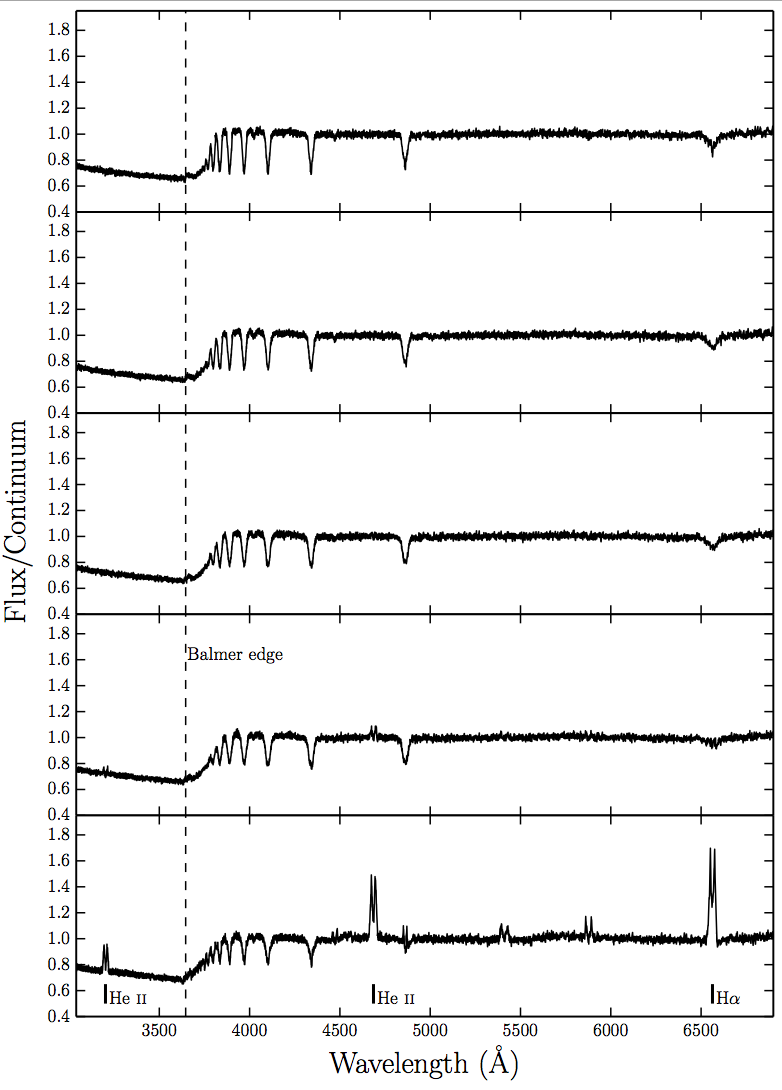
\includegraphics[width=1.0\textwidth]{figures/05-cvpaper/modela_opt_cont.png}
\caption
[Optical synthetic spectra from the benchmark CV model divided by the continuum.]
{Synthetic optical spectra from model A computed for 
sightlines of 10, 27.5, 45, 62.5 and 80 degrees. In these plots
the flux is divided by a polynomial fit to the 
underlying continuum redward of the Balmer edge, so that 
line-to-continuum ratios and the true depth of the
Balmer jump can be shown.}
\label{spec_continuum}
\end{figure} 

\begin{figure} 
\centering
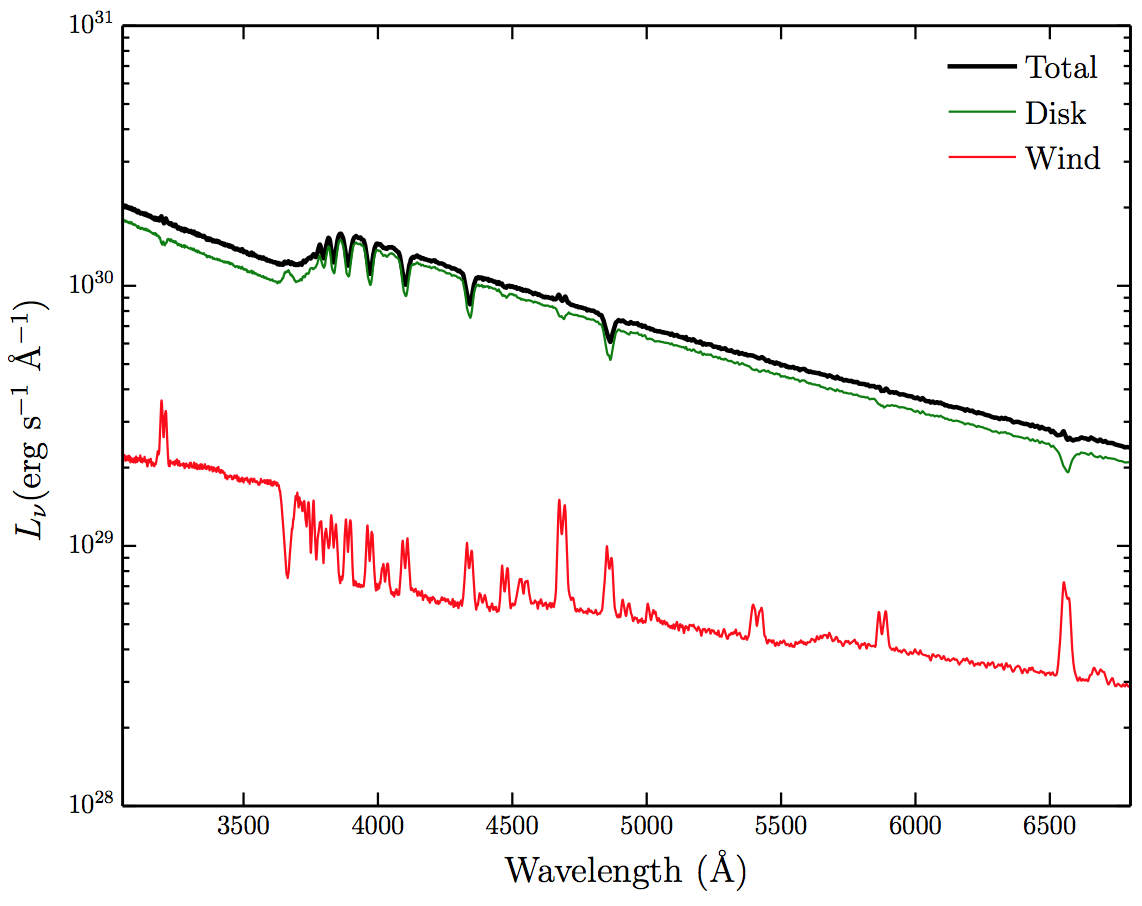
\includegraphics[width=1.0\textwidth]{figures/05-cvpaper/modela_escaping.png}
\caption
[Total packet-binned spectra across all viewing angles from the benchmark CV model.]
{Total packet-binned spectra across all viewing angles, in units
of monochromatic luminosity.
The thick black line shows the total 
integrated escaping spectrum, 
while the green line shows disc photons which escape without being reprocessed by
the wind. The red line show the contributions from reprocessed photons. 
Recombination continuum emission blueward of the Balmer 
edge is already prominent relative to other wind continuum processes, but is not sufficient
to fill in the Balmer jump in this specific model}
\label{cont}
\end{figure} 


%\newpage



%%%%%%%%%%%%%%%%%%%%%%%%%%%%%%%%%%%%%%
%
%          REVISED MODEL
%
%%%%%%%%%%%%%%%%%%%%%%%%%%%%%%%%%%%%%%%

\section{A Revised Model Optimized for Optical Wavelengths}
\label{sec:modelb}
The benchmark model discussed in section~\ref{modela} was originally
designed to reproduce the wind-formed lines seen in the UV spectra of
high-state CVs. This model does produce some observable
optical emission, but I can now attempt to construct a model that more closely 
matches the observed optical spectra of CVs. 

Specifically, I aim to assess whether a revised model can:

\begin{itemize}
         \item account for all of the lines seen in optical spectra 
         of CVs while preserving
the UV behaviour;
         \item produce single-peaked Balmer emission lines; 
         \item generate enough of a wind-formed recombination continuum
to completely fill in the disc's Balmer absorption edge for 
reasonable outflow parameters.
\end{itemize} 

The emission measure of a plasma is directly proportional to its density.
The simplest way to simultaneously affect the density in the wind (for fixed mass-loss rate),
as well as the velocity gradients, is by modifying the poloidal velocity
law. Therefore, I focus on just two kinematic variables:

\begin{itemize}
         \item the acceleration length, $R_v$, which controls the
        distance over which the wind accelerates to $\frac{1}{2}~v_{\infty}$;
         \item the acceleration exponent, $\alpha$, which controls the rate 
         at which the poloidal velocity changes near $R_v$.
\end{itemize} 

The general behaviour we might expect is that outflows with denser
regions near the wind base -- i.e. winds with larger $R_{v}$ and/or
larger $\alpha$ -- will produce stronger optical emission signatures. 
However, this behaviour may be moderated by the effect of the increasing
optical depth through this region, which can also affect the line profile shapes. 
In addition, modifying $R_v$ also increases the emission {\em volume}.
Based on a preliminary exploration of models with different kinematics,
I adopt the parameters listed in table~\ref{modelb_table}
for this new, `optically optimized' model (model B). 

%It is possible that other parameters, such as the launching radii and angles



\subsection{Synthetic Spectra}
\label{sec:modelb_spectra}
\begin{figure*}
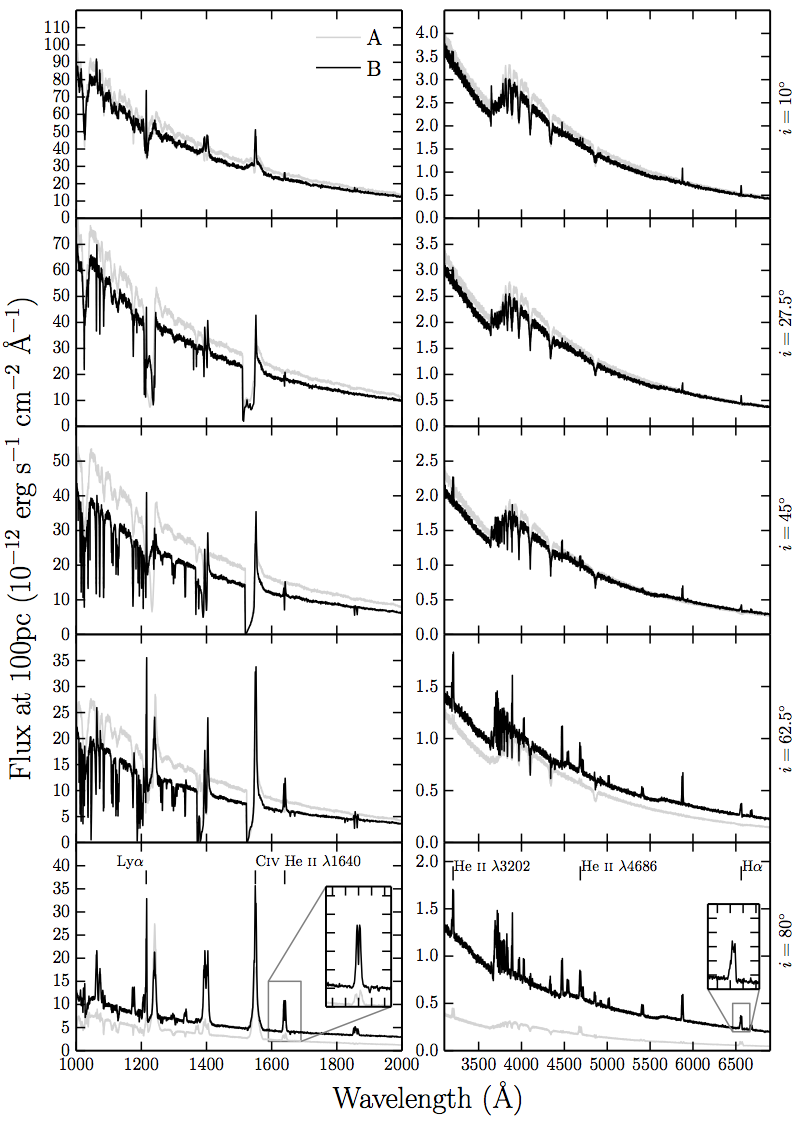
\includegraphics[width=1.0\textwidth]{figures/05-cvpaper/modelb_uv_opt.png}
\caption
[UV and optical synthetic spectra from CV model B]{
UV (left) and optical (right) synthetic spectra for model B computed at
sightlines of 10, 27.5, 45, 62.5 and 80 degrees. 
Model A is shown in grey for comparison.	
The inset plots show zoomed-in line profiles for 
\heiiuv\ and \ha. The Balmer and He
are double-peaked, albeit with narrower profiles.
Strong \heiiopt\ emission can be seen, as well as a trend
of a deeper Balmer jump with decreasing inclination.
}
\label{uvoptb}
\end{figure*}

Fig.~\ref{uvoptb} shows the UV and optical spectra for the
optically optimized model for the full range of inclinations. 
As expected, the trend from absorption to emission 
in the optical is again present, but in this revised model emission
lines in the entire Balmer series are produced at high inclinations, as well
as the observed lines 
in He~\textsc{ii} and He~\textsc{i}. This can be seen more clearly in the 
continuum-normalized spectrum in Fig.~\ref{continuumb}.

Two other features are worth noting in the optical
spectrum. First, the collisionally excited Ca~{\sc ii} emission line at 3934~\AA\ 
becomes quite prominent in the densest models. Second, the model predicts a detectable
He~\textsc{ii} recombination line at 3202~\AA. This is the He
equivalent of Paschen~$\beta$ and should be expected in all systems that
feature a strong He~\textsc{ii}~$\lambda4686$ line (the He
equivalent of Paschen~$\alpha$). 
This line is somewhat unfamiliar observationally, because it 
lies bluewards of the atmospheric cut-off, but
also redwards of most ultraviolet spectra. 

The synthetic spectra do not exhibit P-Cygni profiles in the optical lines.
This is perhaps not surprising. LK02 and SV93 originally designed such models
to reproduce the UV line profiles. Thus, most of the wind
has an ionization parameter of $\log U \sim 2$ (see Fig.~\ref{wind}).
This means H and He are fully ionized throughout 
much of the wind and are successful in producing recombination features.
However, the line opacity throughout the wind is too
low to produce noticeable blue shifted absorption. 
It the systems that exhibit such profiles must 
possess a higher degree of ionization stratification, although the lack 
of contemporary observations means it is not known for certain if the 
P-Cygni profiles in UV resonance lines and optical H and He lines exist simultaneously.
Ionization stratification could be caused by a clumpy flow, in which the 
ionization state 
changes due to small scale density fluctuations, or a stratification in density
and ionizing radiation field over larger scales.
Invoking clumpiness in these outflows is not an unreasonable
hypothesis. Theories of line-driven winds predict an unstable flow
\citep{macgregor1979,owockirybicki1984,owockirybicki1985}, and
simulations of CV disc winds also produce density inhomogeneities 
\citep{proga1998,pkdh2002}.
Tentative evidence for clumping being directly related to P-Cygni optical lines
comes from the fact that \cite{prinja2000}
found the dwarf nova BZ Cam's outflow to be unsteady and highly mass-loaded in outburst,
based on observations of the UV resonance lines.
This system has also exhibited P-Cygni profiles in He~\textsc{i}~$\lambda5876$
and \ha\ when in a high-state \citep{patterson1996,RN98}. 
The degree of ionization and density variation and 
subsequent line opacities may be affected by the model parameters
and the specific parameterisation adopted.

In the UV, the model still produces all the observed lines, 
and deep P-Cygni profiles are produced in the normal resonance lines,
as discussed in section~\ref{sec:modela_spectra}. However, the UV spectra also
display what is perhaps the biggest problem with this revised model,
namely the strength of resonance line emission 
at low and intermediate inclinations.
In order to generate strong optical wind signatures, I have adopted wind
parameters that lead to very high densities at the base of the wind
($n_e\sim10^{13}-10^{14}$~cm$^{-3}$). This produces
the desired optical recombination emission, but also increases the
role of collisional excitation in the formation of the UV resonance
lines. This explains the pronounced increase in the emission component 
of the C\textsc{iv} $\lambda1550$ resonance line, for example, relative to
what was seen in the benchmark model (compare Figures~\ref{spec} and
\ref{uvoptb}). The strength of this component in the revised model 
is probably somewhat too high to be consistent with UV observations 
of high-state CVs (see e.g. Long et al. 1991, 1994; Noebauer et al. 2010).
\nocite{long1991,long1994, noebauer}


\subsection{Continuum Shape and the Balmer Jump}

The wind now also has a clear effect on the continuum shape,
as shown by Fig.~\ref{modelb_escape}. In fact, the majority of the
escaping spectrum has been reprocessed in some way by the wind,
either by electron scattering (the wind is now moderately Thomson-thick),
or by bound-free processes. This is demonstrated by the flatter spectral shape
and the slight He photoabsorption edge present in the optical spectrum 
(marked in Fig.~\ref{continuumb}). This reprocessing is also
responsible for the change in continuum level between models A and B.
In addition, Figures~\ref{uvoptb}, \ref{continuumb} 
and \ref{modelb_escape} clearly demonstrate that the wind produces
a recombination continuum sufficient to completely fill in the Balmer jump
at high inclinations.\footnote{Note that the apparent absorption feature 
just redward of the Balmer jump in these models is artificial. It is
caused by residual line blanketing in the stellar atmospheres, which
the models cannot fill in since they employ a 20-level H atom.}
This might suggest that Balmer continuum emission from a wind can be important 
in shaping the Balmer jump region, as
originally suggested by Knigge et al.
(1998b; see also Hassall et al. 1985)\nocite{KLWB98,hassall}. 

It should be acknowledged, however,
that the Balmer jump in high-state CVs would naturally weaken at
high inclinations due to limb darkening effects \citep{ladous1989, ladous1989b}. 
Although simple limb darkening law which affects 
the emergent flux at each inclination is included,
it is not a {\em frequency dependent} opacity in the model.
As a result, the efficiency of filling in the Balmer jump
should really be judged at low and medium inclinations, 
where, although prominent, the recombination continuum does
not overcome the disc atmosphere absorption. 
In addition, this effect 
could mean that any model which successfully fills in the 
jump at low inclinations could lead to a Balmer jump 
in emission at high inclinations.
In any case, to properly understand this phenomenon, a fully self-consistent
radiative transfer calculation of both the disc atmosphere
and connected wind is required.

\begin{figure} 
\centering
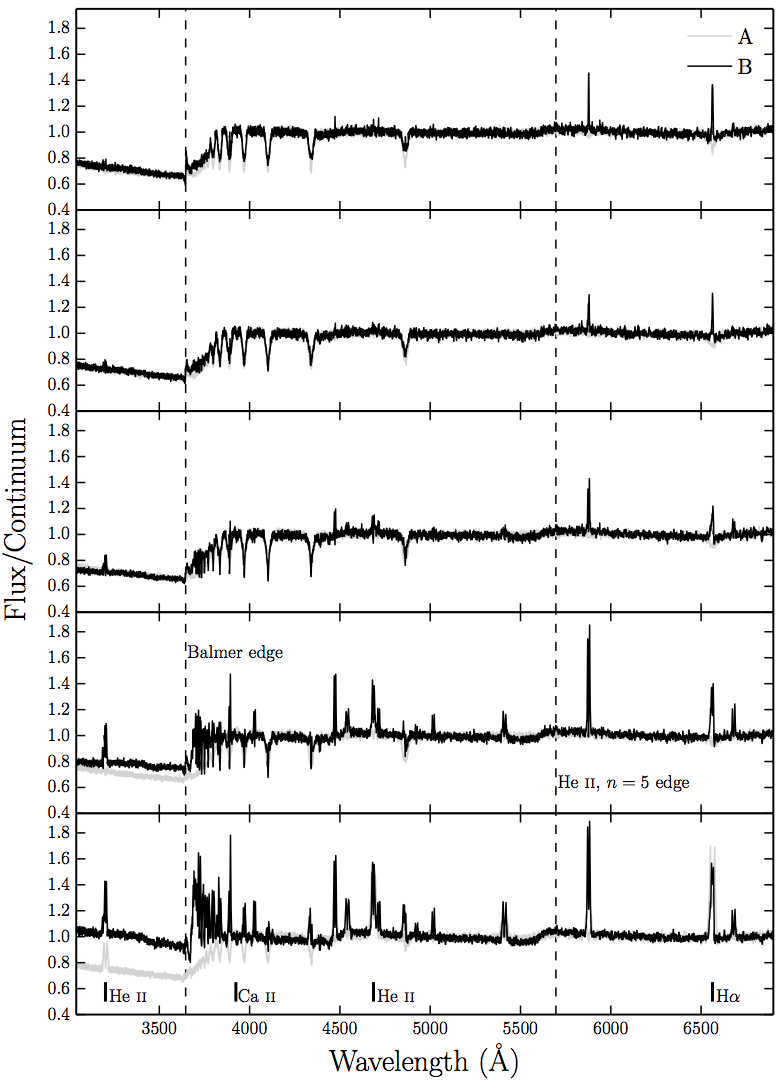
\includegraphics[width=1.0\textwidth]{figures/05-cvpaper/modelb_opt_cont.png}
\caption
[Optical synthetic spectra from CV model B divided by the continuum.]{
Synthetic optical spectra from model B computed for 
sightlines of 10, 27.5, 45, 62.5 and 80 degrees. 
Model A is shown in grey for comparison.
In these plots the flux is divided by a polynomial fit to the 
underlying continuum redward of the Balmer edge, so that 
line-to-continuum ratios and the true depth of the
Balmer jump can be shown.
}
\label{continuumb}
\end{figure} 

\begin{figure} 
\centering
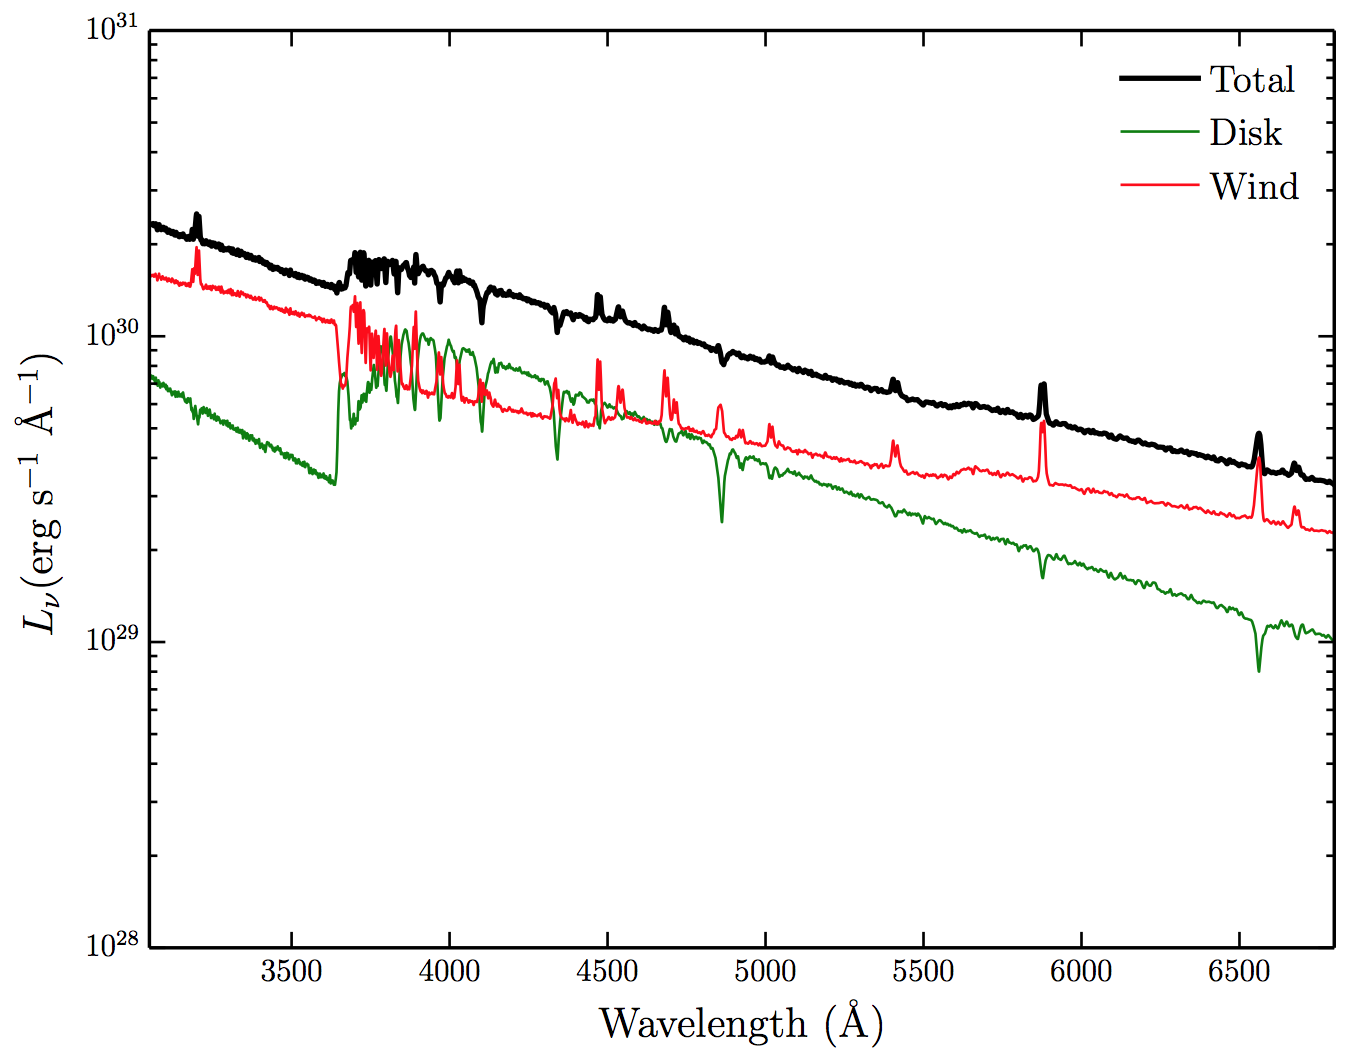
\includegraphics[width=1.0\textwidth]{figures/05-cvpaper/modelb_escaping.png}
\caption
[Total packet-binned spectra across all viewing angles from CV model B.]
{Total packet-binned spectra across all viewing angles, in units
of monochromatic luminosity. 
The thick black line shows the total 
integrated escaping spectrum, 
while the green line shows disc photons which escape without being reprocessed by
the wind. The red line show the contributions from reprocessed 
photons. 
In this denser model the reprocessed contribution is significant compared
to the escaping disc spectrum. The Balmer continuum emission is prominent, and
the wind has a clear effect on the overall spectral shape.}
\label{modelb_escape}
\end{figure} 

\begin{figure}
\centering
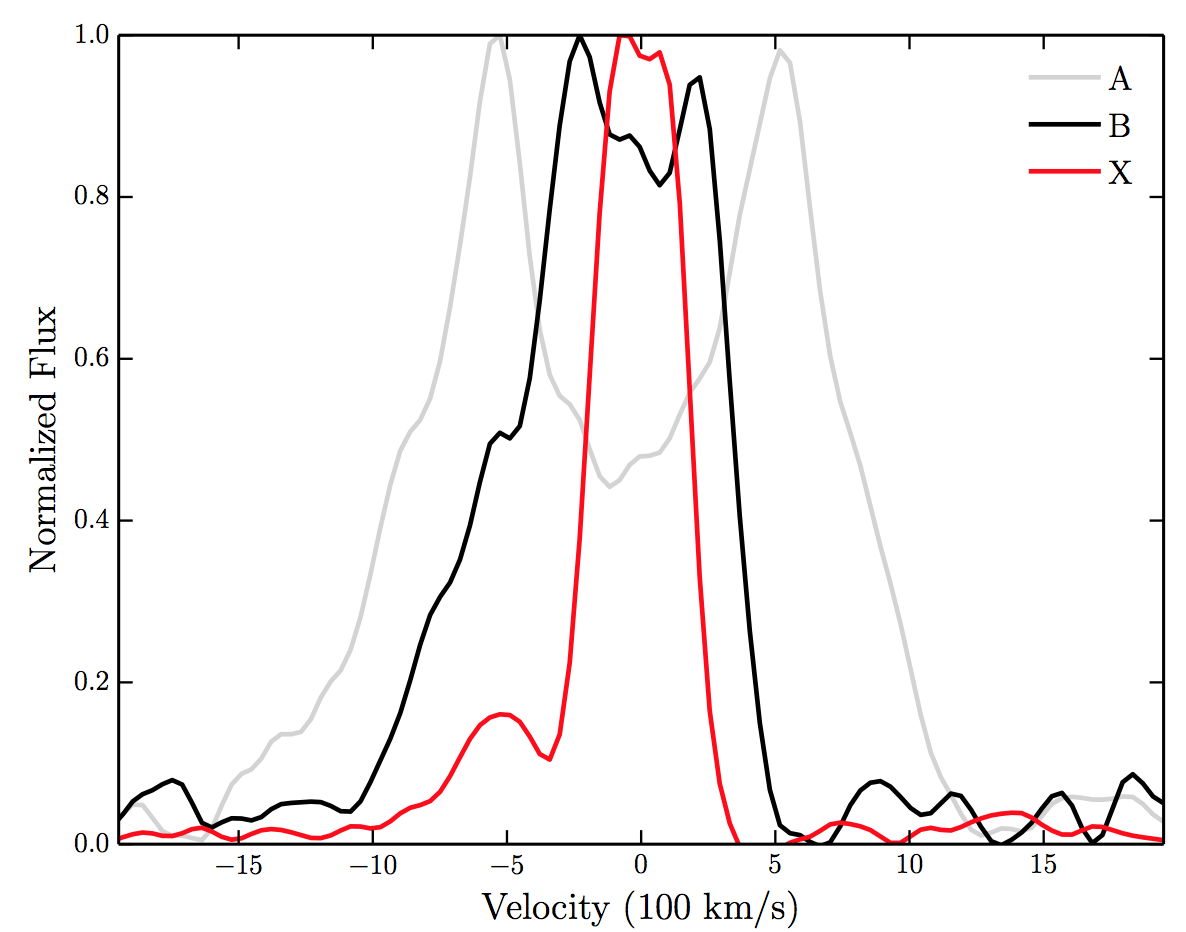
\includegraphics[width=1.0\textwidth]{figures/05-cvpaper/mc.png}
\caption
[\ha\ line profiles from CV models A, B and X]
{
\ha\ line profiles, normalized to 1, plotted in velocity space 
for three models with varying kinematic 
properties, computed at an inclination of $80^\circ$.
The benchmark model and the improved optical
model described in section~\ref{sec:modelb} are labeled as A and B respectively,
and a third model (X) which has an increased acceleration length of 
$R_v = 283.8~R_{WD}$, and $\alpha=4$ is also shown. 
The $x$-axis limits correspond to the Keplerian velocity at 
$4R_{WD}$, the inner edge of the wind.
There is a narrowing of the lines, and a single-peaked line in model X.
This is not due to radial velocity shear (see section~\ref{sec:cv_line_shapes}).
}
\label{halpha}
\end{figure} %fullpage






\subsection{Line Profile Shapes: Producing Single-Peaked Emission}
\label{sec:cv_line_shapes}

Fig.~\ref{halpha} shows how the H$\alpha$ profile changes with the kinematics of the wind for 
an inclination of $80^\circ$. The main prediction is that dense, slowly accelerating 
wind models produce narrower emission lines. This is {\em not} due to radial 
velocity shear. As stated by MC96, that mechanism can only work if poloidal 
and rotational velocity gradients satisfy $(dv_l/dr)/(dv_\phi/dr) \gtrsim 1$; in 
these models, this ratio is always $\lesssim 0.1$. Instead, the narrow lines predicted 
by the denser wind models can be traced to the base of the outflow becoming optically 
thick in the continuum, such that the line emission from the base of the wind
cannot escape to the observer. In such models, the `line photosphere'
(the $\tau \simeq 1$ surface of the line-forming region) moves outwards, towards larger 
vertical and cylindrical distances. This reduces the predicted line widths, since the 
rotational velocities -- which normally provide the main line broadening mechanism at 
high inclination -- drop off as $1/r$. This is not to say that the MC96 
mechanism could not be at work in CV winds. For example, it would be worth investigating
alternative prescriptions for the wind velocity field, as well as the possibility that the 
outflows may be clumped. An inhomogeneous flow 
(which has been predicted in CVs; see section~\ref{sec:modelb_spectra})
might allow large radial velocity shears to exist while still 
maintaining the high densities needed to produce the required level of emission.
However, such an investigation is beyond the scope of the present paper.

In these models, single-peaked line profiles are produced once the line forming region 
has been
pushed up to $\sim 10^{11}$~cm ($\sim150~R_{WD}$) above the disc plane. 
This number may seem unrealistically large, but the vertical extent of 
the emission region is actually not well constrained observationally. 
In fact, multiple observations of eclipsing NLs show that the H$\alpha$ 
line is only moderately eclipsed compared to the continuum (e.g. Baptista et al. 2000;
Groot et al. 2004; see also section~\ref{sec:rwtri}), 
implying a significant vertical extent for the line-forming 
region. This type of model should therefore not be ruled out {\em a priori}, 
but this specific model was not adopted as the optically optimized model
due to its unrealistically high continuum level in eclipse. 

\subsection{Sensitivity to Model Parameters}
\label{sec:cv_params}
This revised model demonstrates that one can achieve a more
realistic optical spectrum by altering just two kinematic parameters. 
However, it may also be possible to achieve this by modifying
other free parameters such as $\dot{M}_{W}$, the opening angles of the wind and the 
inner and outer launch radii. For example, increasing the mass-loss rate of the wind
increases the amount of recombination emission (which scales as $\rho^2$), 
as well as lowering the ionization parameter and increasing the optical depth through the wind. 
Larger launching regions and covering factors tend to lead to a larger emitting volume, 
but this is moderated by a decrease in density 
for a fixed mass-loss rate. I also note that the inner radius of $4~R_{WD}$ adopted by SV93 
affects the emergent UV spectrum seen at inclinations $<\theta_{\mathrm{min}}$ as 
the inner disc is uncovered. This causes less absorption in the UV resonance lines,
but the effect on the optical spectrum is negligible.
I have verified this general behaviour, but
I suggest that future work should investigate the effect of these parameters in more detail,
as well as incorporating a treatment of clumping.
If a wind really does produce the line and continuum emission seen in optical spectra of high-state CVs, then
understanding the true mass-loss rate and geometry of the outflow is clearly important.


\subsection{Comparison to RW Tri}
\label{sec:rwtri}
\begin{figure*}
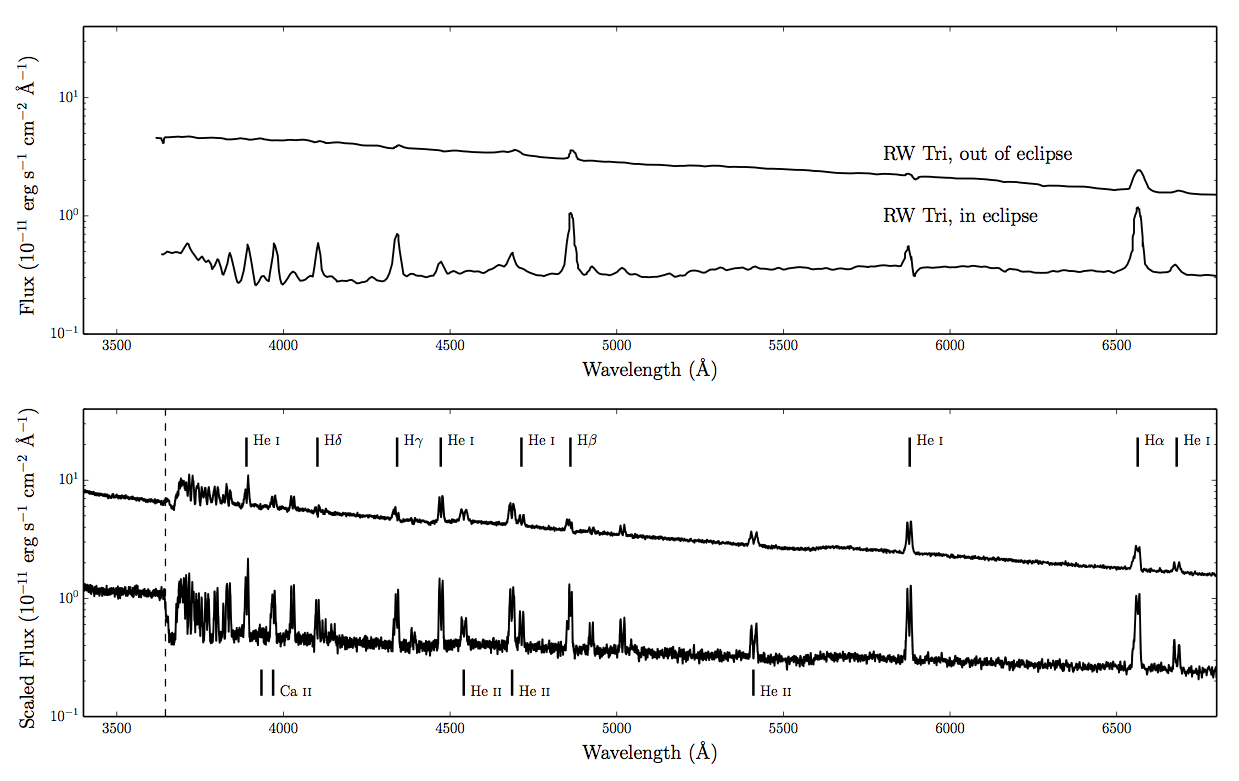
\includegraphics[width=0.9\textheight, angle=270]{figures/05-cvpaper/fig13.png}
\caption
[In and out of eclipse spectra from model B compared to the high
inclination NL RW Tri]
{{\sl Top Panel:} In and out of eclipse spectra of the high
inclination NL RW Tri. {\sl Bottom Panel:} In and out of eclipse synthetic
spectra from model B.
The artificial `absorption' feature just redward of the Balmer jump
is due to the reasons described in section 5.2.}
\label{rwtricomp}
\end{figure*}

Fig.~\ref{rwtricomp} shows a comparison of the predicted
out-of-eclipse and mid-eclipse spectra against observations of the
high-inclination nova-like RW~Tri. The inclination of RW Tri is
somewhat uncertain, with estimates including $70.5^\circ$
\citep{smak1995}, $75^\circ$ \citep{groot2004}, $80^\circ$
\citep{longmore1981} and $82^\circ$\citep{frankking1981}. Here, we
adopt $i = 80^\circ$, but the qualitative conclusions are not
particularly sensitive to this choice. 
I follow LK02 is setting the value of $r_{\mathrm{disc}}(\mathrm{max})$ (the maximum radius of the accretion disc)
to $34.3~R_{WD}$. When compared to the semi-major axis of RW Tri,
this value is perhaps lower than one might 
typically expect for NLs \citep{harropallinwarner1996}. 
However, it is consistent
with values inferred by \cite{rutten1992}.
I emphasize that this model is in no sense a fit to this -- or any other -- data set.


The similarity between the synthetic and observed spectra is
striking. In particular, the revised model produces strong emission in
all the Balmer lines, with line-to-continuum ratios comparable to
those seen in RW Tri. Moreover, the line-to-continuum contrast
increases during eclipse, as expected for emission produced in a disc
wind. This trend is in line with the observations of RW~Tri, and it
has also been seen in other NLs, including members of the SW~Sex class
\citep{neustroev2011}. As noted in section~\ref{sec:modelb_spectra}, the majority
of the escaping radiation has been reprocessed by the wind in some way
(particularly the eclipsed light).

However, there are also interesting differences between the revised
model and the RW Tri data set. For example, the synthetic spectra exhibit
considerably stronger He~{\sc ii} features than the observations,
which suggests that the overall ionization state of the model is
somewhat too high. As discussed in section~\ref{sec:cv_line_shapes}, 
the optical lines are narrow, but double-peaked. 
This is in contrast to what is generally seen in observations
of NLs, although the relatively low resolution of the RW Tri
spectrum makes a specific comparison difficult. In order to demonstrate
the double-peaked nature of the narrower lines, I do not 
smooth the synthesized data to the resolution of the RW Tri dataset.
If the data was smoothed, the \ha\ line would appear single-peaked.

\subsection{A Note on Collision Strengths}
\label{sec:coll_bl}

\py\ uses the \cite{vanregemorter} approximation 
(see section~\ref{sec:coll}) to calculate collision rates.
This approach uses an effective gaunt factor, of
order unity. To conduct these specific simulations a value of $\bar{g}=1$ 
was adopted. There are two main concerns when using this approach.
The first is related to accuracy, as poorly estimating collision strengths
could lead to incorrect heating and cooling balance in the flow, with
knock-on effects on the emergent spectrum. This is of particular concern
here as line heating is the dominant heating mechanism in the dense 
base of the wind. I have verified that the main conclusions of this study
are fairly insensitive to the gaunt factor; for example, if I adopt
$\bar{g}=0.2$ as suggested by, e.g, \citep{ferland2005} than the wind still
produces a host of recombination lines. 
I improved collision strengths reduced the wind temperature it 
could mean that a boundary layer might
actually be required to produce the higher ionization lines such as 
\heiiopt\ \citep[see e.g.][]{hoare1991}.

The second concern is that 
collisions between radiatively forbidden transitions are not taken into 
account when one splits levels into $l$- and $s$-subshells, as well
as principal quantum number, $n$ (as I have done with He~\textsc{i}; 
see section~\ref{sec:atomic_data}). However, I have verified that
in this case the plasma is dense enough that recombination 
dominates the level populations, at least in 
the regions responsible for the optical line emission. In other words, two levels
that are linked only by a forbidden transition have their relative populations
determined their recombination rates from the upper ion.
Nevertheless, for future efforts it would be desirable to include
collisional data for forbidden transitions, an effort that has now
been started (see chapter 7).



% \subsection{Model Sensitivity to Collision Strengths}
% \subsubsection{Collisions Between Radiatively Forbidden Transitions}
% \label{sec:rad_forbid}
% \subsubsection{Line Heating and Cooling}
% \label{sec:line_heat}
% Fig.~?? shows four important heating and cooling mechanisms 
% in the wind for model B. Line heating and cooling 
% \subsection{Improving Collision Strengths}
% \subsection{Introducing a Boundary Layer}



%%%%%%%%%%%%%%%%%%%%%%%%%%%%%%%%%%%%%%
%
%          CONCLUSIONS
%
%%%%%%%%%%%%%%%%%%%%%%%%%%%%%%%%%%%%%%%


\section{Conclusions}
\label{sec:cv_conclusions}

I have investigated whether a disc wind model designed to reproduce
the UV spectra of high-state CVs would also have a significant effect
on the optical spectra of these systems. I find that this is indeed
the case. In particular, the model wind produces H and He
recombination lines, as well as a recombination continuum blueward of
the Balmer edge. The spectra do not show P-Cygni profiles
in the optical H and He lines, which are seen in a small fraction of CV 
optical spectra. Possible reasons for this are briefly discussed in 
section~\ref{sec:modelb_spectra}.

A revised benchmark model was also constructed
to more closely match the optical spectra of high-state CVs. This
optically optimized model produces all the prominent optical lines in
and out of eclipse, and achieves reasonable verisimilitude with the
observed optical spectra of RW Tri. However, this model also has
significant shortcomings. In particular, it predicts
stronger-than-observed He~{\sc ii} lines in the optical region and too
much of a collisionally excited contribution to the UV resonance lines. 
Incorporating more accurate collisional data into \py\ will help
assess this discrepancy in more detail.

Based on these results, I argue that recombination emission 
from outflows with sufficiently high densities and/or optical depths 
might produce the optical lines observed in CVs, and may also 
fill in the Balmer absorption edge in the spectrum of the accretion disc, 
thus accounting for the absence of a strong edge in observed CV spectra.
In section~\ref{sec:cv_line_shapes}, I demonstrated that
although the double peaked lines narrow and 
single-peaked emission can be formed in the densest models, 
this is not due to the radial velocity shear mechanism proposed by MC96.
I suggest that `clumpy' line-driven winds or a different
wind parameterization may nevertheless allow this mechanism to work.
I also note the possibility that, as in the denser models, 
the single-peaked lines are formed well above the disc, where 
rotational velocities are lower.

It is not yet clear whether a wind model such as this can
explain all of the observed optical features of high-state CVs --
further effort is required on both the observational
and modelling fronts. However, this work demonstrates that disc winds may
not just be responsible for creating the blue-shifted absorption and
P-Cygni profiles seen in the UV resonance lines of high-state CVs, but
can also have a strong effect on the optical appearance of these
systems. In fact, most of the optical features characteristic of CVs
are likely to be affected -- and possibly even dominated -- by their disc
winds. Given that optical spectroscopy plays the central role in
observational studies of CVs, it is critical to know 
where and how these spectra are actually formed. I believe it is high
time for a renewed effort to understand the formation of spectra in
accretion discs and associated outflows. 


